\documentclass["../Cours.tex"]{subfiles}

\begin{document}

\centerline{\Huge{Bases numériques}}
\begin{questions}
    \PARTIETITRE{Le système décimal}

    \textit{Nous avons pour habitude d'écrire les nombres en utilisant 10 chiffres (de 0 à 9). Il est souvent admis que ce choix est corrélé à notre nombre de doigts.}

    \question On peut décomposer un nombre selon ses chiffres de la manière suivante : 
    \begin{align*}
        \num{12058} &= \num{10000} + \num{2000} + 50 + 8 \\ 
        &= 1 \times \num{10000} + 2 \times \num{1000} + 5 \times 10 + 8 \times 1 \\ 
        &= 1 \times 10^4 + 2 \times 10^3 + 5 \times 10^1 + 8 \times 10^0
    \end{align*}

    \subquestion Décomposer de la même manière le nombre \num{482005}.
    \subquestion Décomposer de la même manière le nombre \num{1027.163}.

    \PARTIETITRE{Le système binaire}

    \textit{Un ordinateur ne possède pas 10 doigts, c'est pourquoi il n'est pas forcément pertinent d'utiliser 10 chiffres en informatique. Dans un transistor (les très petits composant qui constituent un processeur, ayant une taille aujourd'hui entre \qty{3}{\nano\metre} et \qty{20}{\nano\metre}), soit le courant passe (1), soit le courant ne passe pas (0). Les interrupteurs par exemple utilisent cette notation. }

    \begin{center}
        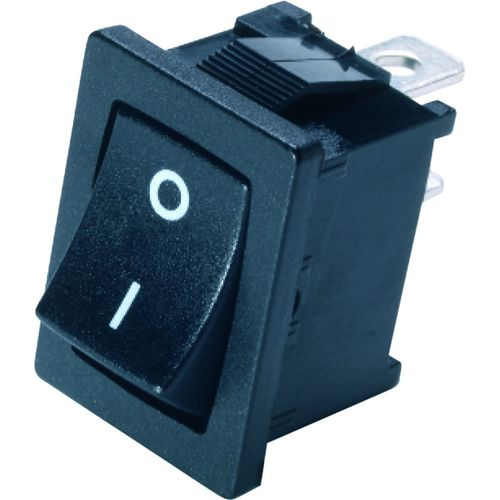
\includegraphics[scale=0.2]{4 - Quatrieme/problemes/72374-9540269.jpg}
        
\begin{tikzpicture}[scale=0.4]
            \fill (-0.5,-0.5) rectangle (0.5,3.5);
            \fill ({3*cos(120)},{3*sin(120)}) arc(120:420:3) -- ({2*cos(60)},{2*sin(60)}) arc(420:120:2) -- cycle;
        \end{tikzpicture}
    \end{center}

    \question On peut décomposer un nombre selon ses chiffres en \emph{base binaire} de la manière suivante : 
    \begin{align*}
        54 &= 32 + 16 + 4 + 2 \\
        &= 2^5 + 2^4 + 2^2 + 2^1 \\
        &= 1 \times 2^5 + 1 \times 2^4 + 0 \times 2^3 + 1 \times 2^2 + 1 \times 2^1 + 0 \times 2^0 \\
        \Aboxed{(54)_{10} &= (110110)_{2}}
    \end{align*}

    \subquestion Décomposer de la même manière 98.
    \subquestion Décomposer de la même manière 537.
    \subquestion Décomposer de la même manière 255.

    \question Calculer $537+255$ en système décimal et en système binaire.

    \PARTIETITRE{Le système hexadécimal}

    \textit{Bien que les 1 et les 0 soient manipulés par les machines, les nombres écrits en système binaire sont souvent trop longs pour que les humains puissent les lire et les manipuler. Pour les raccourcir, on regroupe les paquets de 1 et de 0 par groupe de 4. Ainsi, puisque $2^4=16$, il y aura 16 chiffres (de 0 à 9, puis A, B, C, D, E, F).}

    \begin{multicols}{4}
        \begin{itemize}
            \item \( (0)_{16} = (0000)_2 \)
            \item \( (1)_{16} = (0001)_2 \)
            \item \( (2)_{16} = (0010)_2 \)
            \item \( (3)_{16} = (0011)_2 \)
            \item \( (4)_{16} = (0100)_2 \)
            \item \( (5)_{16} = (0101)_2 \)
            \item \( (6)_{16} = (0110)_2 \)
            \item \( (7)_{16} = (0111)_2 \)
            \item \( (8)_{16} = (1000)_2 \)
            \item \( (9)_{16} = (1001)_2 \)
            \item \( (A)_{16} = (1010)_2 \)
            \item \( (B)_{16} = (1011)_2 \)
            \item \( (C)_{16} = (1100)_2 \)
            \item \( (D)_{16} = (1101)_2 \)
            \item \( (E)_{16} = (1110)_2 \)
            \item \( (F)_{16} = (1111)_2 \)
        \end{itemize}
    \end{multicols}

    \question Le nombre $(0101~1011~1110~0010)_2$ s'écrit $(5BE2)_{16}$.
    \subquestion Écrire en système hexadécimal $(1001~1011~0010~0000)_2$.
    \subquestion Écrire en système hexadécimal $(0111~1010~0110~0111)_2$.
    \subquestion Écrire en système hexadécimal $(0010~1100~1110~0100)_2$.
    \subquestion Écrire en système hexadécimal $(0000~1100~0110~0110)_2$.

    \question On peut trouver la valeur décimale d'un nombre en système hexadécimal de la manière suivante : 
    \begin{align*}
        (5BE2)_{16} &= 5 \times 16^3 + 11 \times 16^2 + 14 \times 16^1 + 2 \times 16^0 \\
        &= 5 \times 4096 + 11 \times 256 + 14 \times 16 + 2 \times 1 \\ 
        &= 20480 + 2816 + 224 + 2 \\ 
        &= 23522
    \end{align*}
    \subquestion Écrire en système décimal $(10)_{16}$.
    \subquestion Écrire en système décimal $(3A)_{16}$.
    \subquestion Écrire en système décimal $(AF2C)_{16}$.

    \PARTIETITRE{Combinatoire}
    \question Si on écrit un code à 4 chiffres en système décimal, il y aura 10 possibilités pour le premier chiffre (0 à 9), 10 possibilités pour le deuxième, 10 pour le troisième, 10 pour le quatrième. Au total, il y aura 
    \[ 10 \times 10 \times 10 \times 10 = 10^4 = \num{10000} \]

    C'est assez logique, en effet le premier nombre possible est 0000, puis 0001, jusqu'à 9999. Il y en  a donc bien 10000.

    \subquestion Si on écrit un code en système décimal à 8 chiffres, combien y a-t-il de combinaisons possibles ?
    \subquestion Un voleur teste 1 combinaison par seconde, combien de temps lui faudra-t-il pour tester toutes les combinaisons ?
    \subquestion Un ordinateur teste 10 million de combinaison par seconde, combien de temps lui faudra-t-il pour tester toutes les combinaisons ?

    \question Si on écrit un code en système binaire à 10 chiffres, combien y a-t-il de combinaisons possibles ?
    \question Si on écrit un code en système hexadécimal à 8 chiffres, combien y a-t-il de combinaisons possibles ?
    \question \textit{Le SIV (Système d'Immatriculation des Véhicules) utilisé actuellement est entré en vigueur le 15 avril 2009 en France. Chaque véhicule a une série de lettres et de chiffres décimaux inscrit sur une \emph{plaque d'immatriculation} à l'avant et à l'arrière du véhicule. Elle se doit de respecter les règles suivantes : 
    \begin{itemize}
        \item L'immatriculation est composée de 2 lettres, puis 3 chiffres, puis 2 lettres (par exemple : AB-123-CD)
        \item Les 3 chiffres du milieu vont de 001 à 999 (donc il n'est pas possible d'avoir 000 au milieu)
        \item Les lettres I, O, U sont interdites.
        \item Il ne peut pas y avoir "SS" à gauche ou à droite.
        \item Il ne peut pas y avoir "WW" à gauche. (lettres réservées pour les plaques temporaires)
    \end{itemize}
    }
    $\longrightarrow$ Combien de plaques d'immatriculations sont possibles ?

    \clearpage
    \PARTIETITRE{Couleurs en informatique}
    \textit{La rétine de nos yeux est tapissée de capteurs de couleurs, appelés \emph{cônes}, et - pour la plupart des êtres humains - il en existe 3 types : rouge, vert et bleu (du plus fréquent au moins fréquent). Ces couleurs sont appelées \emph{couleurs primaires.}}

    \textit{Un écran attribue une valeur entre 0 et 255 à chaque couleur primaire. Si on veut afficher du rouge pur, on écrira le code RVB (Rouge Vert Bleu) << \#FF0000 >> en hexadécimal. Les deux premiers chiffres $(FF)_{16} = (255)_{10}$ correspondent au rouge, les deux du milieu $(00)_{16}=(0)_{10}$ au vert et les deux de droite $(00)_{16}=(0)_{10}$ au bleu. }

    \question Le drapeau français est tricolore : << bleu france >>, blanc et << rouge marianne >>. 
    \begin{flushright}\vspace{-1ex}
        (source : \scriptsize{https://www.gouvernement.fr/charte/charte-graphique-les-fondamentaux/les-couleurs})
    \end{flushright}\vspace{-1ex}
    \subquestion Donner le code hexadécimal du << bleu france >> (0, 0, 145).
    \subquestion Donner le code hexadécimal du blanc (255, 255, 255).
    \subquestion Donner le code hexadécimal du << rouge marianne >> (225, 0, 15).

    \question Quel code hexadécimal correspond au noir ?
    \question Quelle est la particularité des codes hexadécimaux des différentes valeurs de gris ?

    \PARTIETITRE{Base 64}
    \textit{Chaque vidéo sur Youtube a un code qui lui est attribué au moment de sa mise en ligne, constitué de 11 caractères en base 64 (0 à 9, puis A à Z (majuscules), puis a à z (minuscules), - et \_). On la retrouve dans l'URL de la vidéo après le << v >> : https://www.youtube.com/watch?v=\textbf{gocwRvLhDf8}.}

    \question Donner en écriture scientifique le nombre de vidéos possibles avec ce système.
    \question Selon le support de Youtube, au maximum une vidéo ne peut être plus longue que \qty{12}{\hour}, quelle durée de vidéos Youtube peut stocker au maximum avec ce système ? Donner la réponse en années.
    \begin{flushright}\vspace{-1ex}
        (source : \scriptsize{https://support.google.com/youtube/answer/71673?hl=fr})
    \end{flushright}\vspace{-1ex}
    \question Sachant que le Big Bang a eu lieu il y a environ \qty{13.8e9}{années}, conclure sur l'efficacité de ce système.
        \begin{flushright}\vspace{-1ex}
        (source : \scriptsize{https://doi.org/10.48550/arXiv.astro-ph/0603449})
    \end{flushright}\vspace{-1ex}

\end{questions}

\end{document}